In the first lecture, we derived a model for a suspension system
\begin{center}
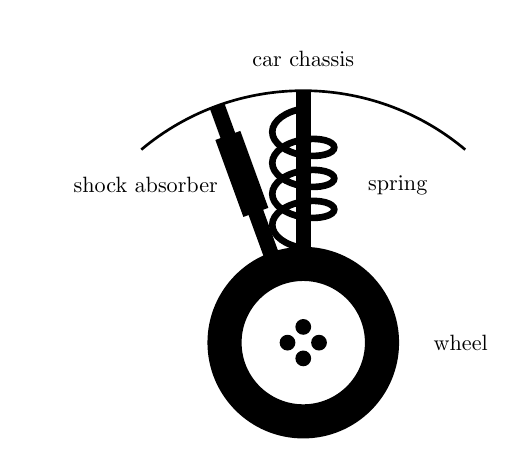
\begin{tikzpicture}[scale=1,inner sep=0pt,outer sep=0pt,very thick]

\useasboundingbox (-3.5,-1) rectangle (2.5,4); 
\begin{scope}[transform canvas={scale=.8}]
\draw[line width=3pt,decorate,decoration={coil,segment length=14,amplitude=14}] (0,1.5) -- (0,4);
\draw[line width=7pt] (0,0) -- (0,4);
\draw (1.5,2.5) node {spring};

\draw[line width=7pt,rotate=20] (0,0) -- (0,4);
\draw[line width=12pt,rotate=20] (0,2.2) -- (0,3.5);
\draw (-2.5,2.5) node {shock absorber};

\draw (0,0) node[draw,fill=black,circle,minimum width=3cm] {};
\draw (0,0) node[draw,fill=white,circle,minimum width=2cm] {};
\draw (.25,0) node[fill=black,circle,minimum width=.25cm] {};
\draw[rotate=90] (.25,0) node[fill=black,circle,minimum width=.25cm] {};
\draw[rotate=180] (.25,0) node[fill=black,circle,minimum width=.25cm] {};
\draw[rotate=-90] (.25,0) node[fill=black,circle,minimum width=.25cm] {};
\draw (2.5,0) node {wheel};

\draw (50:4) arc (50:130:4);
\draw (0,4.5) node {car chassis};
\end{scope}

\end{tikzpicture}
\hspace{.25in}
\begin{tikzpicture}

\draw[inner sep=0pt,outer sep=0pt,very thick] (0,-2) node[rotate=90,draw,circle,minimum width=1pt] (gnd1) {};
\draw[inner sep=0pt,outer sep=0pt,very thick] (1,0) node[rotate=90] (K1) {\begin{tikzpicture}
\draw (.75,0) node[inner sep=0,outer sep=0] (K1) {\begin{tikzpicture}
\draw (.75,0) node[inner sep=0,outer sep=0] (K1) {\begin{tikzpicture}
\draw (.75,0) node[inner sep=0,outer sep=0] (K1) {\input{\mainfolder/DrawingElements/MechanicalElements/spring.tex}};
\draw (K1)  node[above=6pt] {$k$};
\draw[very thick] (K1.180) -- ++(-.2,0);
\draw[very thick] (K1.0) -- ++(0.2,0);
\draw[<-,thick] (K1.0) ++(.2,0) -- ++(.5,0) node[right] {$f$};
\draw[<-,thick] (K1.180) ++(-.2,0) -- ++(-.5,0) node[left] {$f$};
\draw[|->,thick] (K1.180) ++(-.2,.4) node[above=2pt] {$x_{1}$} -- ++(.5,0);  
\draw[|->,thick] (K1.0) ++(.2,.4) node[above=2pt] {$x_{2}$} -- ++(.5,0);  
\draw<2-> (K1) ++(0,-.6) node {$f=k(x_{1}-x_{2})$};
\end{tikzpicture}
};
\draw (K1)  node[above=6pt] {$k$};
\draw[very thick] (K1.180) -- ++(-.2,0);
\draw[very thick] (K1.0) -- ++(0.2,0);
\draw[<-,thick] (K1.0) ++(.2,0) -- ++(.5,0) node[right] {$f$};
\draw[<-,thick] (K1.180) ++(-.2,0) -- ++(-.5,0) node[left] {$f$};
\draw[|->,thick] (K1.180) ++(-.2,.4) node[above=2pt] {$x_{1}$} -- ++(.5,0);  
\draw[|->,thick] (K1.0) ++(.2,.4) node[above=2pt] {$x_{2}$} -- ++(.5,0);  
\draw<2-> (K1) ++(0,-.6) node {$f=k(x_{1}-x_{2})$};
\end{tikzpicture}
};
\draw (K1)  node[above=6pt] {$k$};
\draw[very thick] (K1.180) -- ++(-.2,0);
\draw[very thick] (K1.0) -- ++(0.2,0);
\draw[<-,thick] (K1.0) ++(.2,0) -- ++(.5,0) node[right] {$f$};
\draw[<-,thick] (K1.180) ++(-.2,0) -- ++(-.5,0) node[left] {$f$};
\draw[|->,thick] (K1.180) ++(-.2,.4) node[above=2pt] {$x_{1}$} -- ++(.5,0);  
\draw[|->,thick] (K1.0) ++(.2,.4) node[above=2pt] {$x_{2}$} -- ++(.5,0);  
\draw<2-> (K1) ++(0,-.6) node {$f=k(x_{1}-x_{2})$};
\end{tikzpicture}
};
\draw (1,0) node[right=14pt] {$k$};
\draw[inner sep=0pt,outer sep=0pt,very thick] (-1,0) node[rotate=90] (D1) {\begin{tikzpicture}
\draw[very thick] (-.2,0) -- (0,0);
\draw (.75,0) node {\begin{tikzpicture}
\draw[very thick] (-.2,0) -- (0,0);
\draw (.75,0) node {\begin{tikzpicture}
\draw[very thick] (-.2,0) -- (0,0);
\draw (.75,0) node {\input{\mainfolder/DrawingElements/MechanicalElements/damper.tex}};
\draw (.75,0) node[above=9pt] {$b$};
\draw[very thick] (1.5,0) -- ++(.2,0);
    \draw[<-,thick] (1.5,0) ++(.2,0) -- ++(.5,0) node[right] {$f$};
    \draw[<-,thick] (-.2,0) -- ++(-.5,0) node[left] {$f$};
    \draw[|->,thick] (-.2,.4) node[above=2pt] {$x_{1}$} -- ++(.5,0);  
    \draw[|->,thick] (1.7,.4) node[above=2pt] {$x_{2}$} -- ++(.5,0);  
    \draw (.6,-.6) node {$x=x_{1}-x_{2}$};
  %  \draw (.6,-1.2) node {$f=b\dot{x}$};
\end{tikzpicture}};
\draw (.75,0) node[above=9pt] {$b$};
\draw[very thick] (1.5,0) -- ++(.2,0);
    \draw[<-,thick] (1.5,0) ++(.2,0) -- ++(.5,0) node[right] {$f$};
    \draw[<-,thick] (-.2,0) -- ++(-.5,0) node[left] {$f$};
    \draw[|->,thick] (-.2,.4) node[above=2pt] {$x_{1}$} -- ++(.5,0);  
    \draw[|->,thick] (1.7,.4) node[above=2pt] {$x_{2}$} -- ++(.5,0);  
    \draw (.6,-.6) node {$x=x_{1}-x_{2}$};
  %  \draw (.6,-1.2) node {$f=b\dot{x}$};
\end{tikzpicture}};
\draw (.75,0) node[above=9pt] {$b$};
\draw[very thick] (1.5,0) -- ++(.2,0);
    \draw[<-,thick] (1.5,0) ++(.2,0) -- ++(.5,0) node[right] {$f$};
    \draw[<-,thick] (-.2,0) -- ++(-.5,0) node[left] {$f$};
    \draw[|->,thick] (-.2,.4) node[above=2pt] {$x_{1}$} -- ++(.5,0);  
    \draw[|->,thick] (1.7,.4) node[above=2pt] {$x_{2}$} -- ++(.5,0);  
    \draw (.6,-.6) node {$x=x_{1}-x_{2}$};
  %  \draw (.6,-1.2) node {$f=b\dot{x}$};
\end{tikzpicture}};
\draw (-1,0) node[left=14pt] {$b$};
\draw (0,2) node[draw,rectangle,minimum width=1.5cm,minimum height=1.5cm,very thick] (M1) {$m_{c}$};

\draw[|->] (gnd1) ++(.5,0) node[right] {$x_{r}$} -- ++(0,.5);
\draw[|->] (M1) ++(1.25,0) node[right] {$x_{c}$} -- ++(0,.5);

\draw[very thick] (K1.180) -- ++(0,-.25) -| (gnd1.0);
\draw[very thick] (D1.180) -- ++(0,-.25) -| (gnd1.0);
\draw[very thick] (K1.0) -- ++(0,.25) -| (M1.-90);
\draw[very thick] (D1.0) -- ++(0,.25) -| (M1.-90);


\end{tikzpicture}
\end{center}
\begin{enumerate}
\item Let $m_{c} = 250 $kg, $b=400$ Ns/m, $k=1000$ N/m. Find the transfer function $\frac{X_{c}(s)}{X_{r}(s)}$. 
\item Suppose the car goes over roads that result in the following trajectories for $x_{r}(t)$. Find the steady state response for $x_{c}(t)$.
\begin{enumerate}
\item $x_{r}(t) = 0.1\cos(.1 t)$
\item $x_{r}(t) = 0.1\cos(1 t)$
\end{enumerate}
\end{enumerate}
